\desmos{ntx79bxwse}{100}{600}
\begin{image}
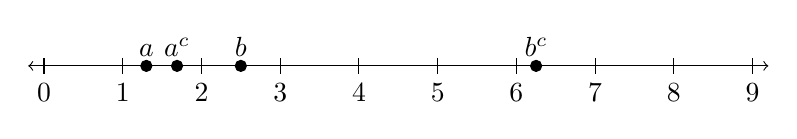
\begin{tikzpicture}
    \draw[<->] (-0.2, 0) -- (9.2, 0);

    \foreach \x in {0, 1, 2, 3, 4, 5, 6, 7, 8, 9} {
        \draw (\x, -0.1) -- (\x, 0.1);
        \node[below] at (\x, -0.1) {$\x$};
    }
    \filldraw[black] (1.3, 0) circle (2pt) node[above]{$a$};
    \filldraw[black] (2.5, 0) circle (2pt) node[above]{$b$};
    \filldraw[black] (6.25, 0) circle (2pt) node[above]{$b^c$};
    \filldraw[black] (1.69, 0) circle (2pt) node[above]{$a^c$};

    \end{tikzpicture}
\end{image}

A number line displaying the relationship between \(a,\) \(b,\) \(a^c,\) and \(b^c.\)